\input{preamble}

\begin{document}
\begin{CJK*}{UTF8}{bsmi}

% \graphicspath{ {./image/} }

\title{Data Structure Homework \#1 \\ Binary Parity Checksum Validator \\with XOR Operator Trained by \\  Neural Network}
\author{Ping-Chen,Chung(鍾秉辰)\\Student ID: 110503007\\Department of Communication Engineering\\National Central University}

	\maketitle
	\tableofcontents
	\newpage
	\begin{abstract}
	This report introduces the basic structure of neural networks and the C functions of dynamic memory allocation, which is used to precisely manage the memory of the program of neural network XOR operator training program. The program then implements the learnt result to calculate the binary parity checksum of an user-input string. The author then analyzed the graph of the loss function(MSE loss) and proposed the further improvement of this program. 
	    
	\end{abstract}
	\section{Theoretical Background of Neural Network}
    In this section, we're going to introduce the definition of neural networks, and its implementations in C as a library.
	\subsection{Neurons}
	Neurons are the fundamental part of the neural network, and they simulate the real neuron from organisms. To turn neuron into a math model, Scientists has given the specific definition and functions of neurons.   
	
	\begin{figure}[h]
	    \centering
	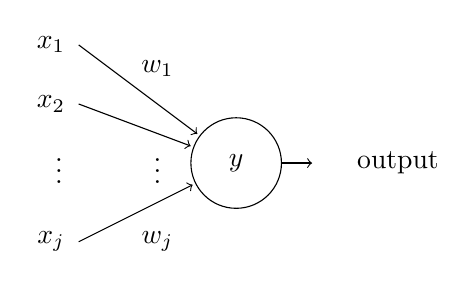
\begin{tikzpicture}[shorten >=1pt,->]
		\tikzstyle{unit}=[draw,shape=circle,minimum size=1.15cm]
 
		\node[unit](p) at (2,1){$y$};
		\node(dots) at (-0.25,1){\vdots};
		\node(dots2) at (1,1){\vdots};
		\node(w1) at (1.0,2.2){$w_1$};
		\node(wj) at (1.0,0){$w_j$};
 
		\draw (0,2.5) node[xshift=-10]{$x_1$} -- (p);
		\draw (0,1.75) node[xshift=-10]{$x_2$} --(p);
		\draw (0,0) node[xshift=-10]{$x_j$} -- (p);
		\draw (p) -- (3,1) node[xshift=30]{output};
% 		\draw (1.2,2.2) node[xshift=-10]{$w_1$};
	\end{tikzpicture}
	    \caption{Model of Neuron \cite{ref4}}
	    \label{fig:my_label}
	\end{figure}
	
	Since the actual neuron in real life sends electric signals only if the inputs have reached  specific conditions, we modeled it to be the \emph{threshold} of the neuron to activate and send a signal to neurons in the next layer. \emph{Weight} is then applied to every input to adjust the importance of each input, and the neuron only activates if the total sum of every input multiplied by its weight is greater than the threshold. The mathematical function of a neuron is given below:
	\begin{eqnarray}
  \mbox{output} & = & \left\{ \begin{array}{ll}
      0 & \mbox{if } \sum_j w_j x_j \leq \mbox{ threshold} \\
      1 & \mbox{if } \sum_j w_j x_j > \mbox{ threshold}
      \end{array} \right.
      \label{percep}
\end{eqnarray}
	Equation \ref{percep} shows one type of neurons: the perceptrons. However, in the modern model of neural networks, we use Sigmoid functions or Softmax functions with other approximating techniques to evaluate neuron outputs to imporve the accuracy of the trained model.   
	\subsection{Network of Neurons}
	As figure \ref{fig:nn-graph} shows, each neuron of the same layer is connected to every node of the next layer, therefore the output of this model can be transformed into matrix form:\\
	\paragraph{Matrixlization of Neuron Networks \cite{ref5}\\}
	Let $x$ inputs be numbered $i_1, i_2, \cdots i_x$, then matrix \textbf{I} is the matrix storing $1\times x$ elements of inputs in the same layer. 
	Each input neuron has its $y$ weights respectively points towards $y$ neurons of the next layer, then the total of input weight is represented by an $x\times y$ matrix \textbf{W}. Multiply \textbf{I} and \textbf{W} gets the inputs of the $y$  neuron in the next layer, stored in $ y\times 1$ matrix \textbf{H}. \\
	The same method can be done repetitively until the output layer is reached. 

 \begin{figure}[h!]
     \centering
    \input{tikz_neuron_net}
     \caption{An Example of Neural Network}
     \label{fig:nn-graph}
 \end{figure}

	\newpage
		\section{Techniques and Resources}
	In this section, we want to introduce a useful concept called \emph{dynamic memory allocation}, and compare it with the known static memory allocation. We also mention the function library \emph{genann} to use, for its simplicity to include. 
 	\subsection{Dynamic Memory Allocation in C}
	    \subsubsection{Difference of Static and Dynamic Memory Allocation }
	    According to reference \cite{ref1}, the author has concluded the advantages and disadvantages of static memory allocation and dynamic memory allocation, shown below:
	    \paragraph{Static Memory Allocation}
	    \begin{itemize}
	        \item Allocation of memory is done automatically by the compiler. This will reduce the execution time of the program.
	        \item Uses stack data structures.
	        \item Allocated memory (including variables and arrays) cannot be freed until the program terminates.
	        \item Memory is allocated before the script executes.
	        \item Simple usage and easy for new learners to use.
	    \end{itemize}
	    \paragraph{Dynamic Memory Allocation}
	    \begin{itemize}
	        \item Memory is allocated in runtime. Hence, the execution time will be increased.
	        \item Uses heap data structures.
	        \item Memory can be resized/freed by scripts, therefore lessening wasted memory in the program.
	        \item Memory should be freed manually after use, or it could cause unknown problems to debug.  
	        \item Needs better knowledge of memory allocation to prevent unknown errors.
	        
	    \end{itemize}
	   
	    \subsubsection{Usable Functions to Dynamically Allocate Memory}
	    \begin{itemize}
	        \item \lstinline{malloc()} allocates the dynamic memory without the initialization. 
	        \item \lstinline{calloc()} allocates the dynamic memory with initialization to prevent accidentally accessing  corrupted memory. 
	        \item \lstinline{realloc()} reallocates the existing memory to expand/shrink its memory size.
	        \item \lstinline{free()} frees the memory and let it be recycled by the operating system.
	    \end{itemize}
	     
	    \subsection{Function Libraries Used in This Program}
	    In this program, we used an open-sourced neural network library Genann \cite{ref2}, with a small number of function library file to include and clear documentation for users to embed into their codes.    
\newpage
		\section{Program}
	This section contains the introduction of some parameters and self-defined functions to make users feel free reading source code. 
	\subsection{Macro-Defined Constants}
	\begin{table}[ht]
	    \centering
	    \begin{tabular}{|l|l|l|}
	    \hline
	        Name  &  Description & Default Value\\
	         \hline
    	     ANN\_INPUT\_NUM &  numbers of inputs in NN model &2\\ 
    	     ANN\_HIDDEN\_LAYERS & numbers of hidden layers in NN  model &1\\ 
    	     ANN\_NEURONS\_PER\_LAYER &  neurons per layer in NN model &2\\ 
    	     ANN\_OUTPUT\_NUM & numbers of inputs in NN model &1\\ 
    	     ANN\_LEARNING\_RATE & the learning rate of neural network &3\\ 
    	     LOOKUP\_SIZE & temporary data storage for \textit{genann}  &4096\\ 
    	     MAX\_CHAR\_LEN & maximum limit of user string input &100\\ 
    	     ZERO\_ASCII & value of 0 in ASCII &48\\ 
    	     TRAIN\_SETS & sets of neural network training
    	     &4\\ 
    	      \hline
	    \end{tabular}
	    \caption{Table of Macro-Defined Constants}
	    \label{tab:my_label}
	\end{table}
	\subsection{Self-Defined Functions}
	\paragraph{void init();\\}
	This function initializes the space of the neural network's lookup size and array sample I/Os for later usage. 
	\paragraph{int selectMode();\\}
	This function asks the user to switch between functions by entering numbers corresponding to the functions by the instruction.
	The function will return an integer representing the enumeration code of functions.   
	\paragraph{char *getInput();\\}
	This function works when the user is asked to enter a string to show its checksum. The function will return the address of the stored string.
	\paragraph{void nnQuadraticLoss(int iteration, int lossReprtSteps);\\}
	This function is used to train the model and display loss function (MSE) based on the given parameters:
	\begin{itemize}
	    \item \lstinline{int iteration} : the number of iteration times to train this model.
	    \item \lstinline{int lossReportSteps} : the interval of generating a report (a line of output in console) of loss. 
	\end{itemize}
	For instance, if we use  \lstinline{nnQuadraticLoss(30000,1000);} , we will get  30000 times of model training and a report in every 1000 epochs.
	\paragraph{void nnTrain(int iteration);\\}
	This function trains the model without showing the loss function. 
	\paragraph{void getBitString(char *string);\\}
	This function generates a string of bits based on the  string user gives. The function will generate a string of bits and call the following function:
	\begin{itemize}
	    \item \textbf{void getRealAns(char *string);} prints the binary parity checksum based on the pre-built XOR operator on the standard library. 
	    \item \textbf{void getTrainAns(char *string);} prints the binary parity checksum based on learned results.  
	\end{itemize}
	
	
	
	\paragraph{void calloc2dArray(double **array, int row, int col);\\}
	This function creates a 2-dimensional array based on the given parameters:
	\begin{itemize}
	    \item \lstinline{double **array} : the address of the 2-dimensional array.
	    \item \lstinline{int row, int col} : the rows and columns of the array. 
	\end{itemize}
	\paragraph{bool nnXor(char num1, char num2);\\}
	    This function takes two characters (only 0 and 1 are allowed) and maps the inputs to the corresponding outputs from learned results.

	\subsection{Compile Parameters}
	    Please open the project directory in command line and execute the following command:
	    \begin{lstlisting}[language=Bash,caption=Compile Parameters]
$ make main 
$ ./main	     \end{lstlisting}
	    \begin{lstlisting}[language=Bash,caption=Compile Results]
cc -Wall -Wshadow -O3 -g -march=native   -c -o main.o main.c
cc   main.o genann.o commonFunctions.o  -lm -o main	     \end{lstlisting}
Note that the warnings from the compiler has been omitted for concise. \newpage
		\section{Execution Results}
	Below is one sample I/O of the program. Note that the input with \lstinline{>>} is user input. 
	 \begin{lstlisting}[language=,caption=Main Program Execution Result]
Welcome to this program. Please choose the mode you want to execute this program.
Enter 1 to show quadratic loss of the training process.
Enter 2 to enter custom string and show the XOR checksum based on NN learning output.
>>2
Please enter the training iteration. (integer)
The training result would be better if trained for 5000 times for 1 layer with 2 nodes per layer.
>>5000
Training Result: 0 1 1 0 
If the result is not "0 1 1 0 ", please consider increase the iteration count or try rerun this program.
Please enter a string. This Program will output the XOR checksum of this string.
>>test_string

Checksum by XOR operator: 0
Checksum generated by neural network: 0   \end{lstlisting}
% \newpage\newpage
	\input{5_Analysis}



	
	
	
    % \bibliographystyle{alpha}
% 	\bibliography{ref}




	\begin{thebibliography}{99}  
	\bibitem{ref4} http://neuralnetworksanddeeplearning.com/chap1.html\\
	
		\bibitem{ref5}https://ml-cheatsheet.readthedocs.io/en/latest/forwardpropagation.html
		\bibitem{ref1}https://www.geeksforgeeks.org/static-and-dynamic-memory-allocation-in-c/
	\bibitem{ref2}https://github.com/codeplea/genann

	\bibitem{ref3}https://www.statlect.com/glossary/loss-function/
		
		
			%\bibitem{ref4}
	
		
	\end{thebibliography} 


\end{CJK*}

\end{document}